
This section deals two complementary scheduling strategies in detail with the performance plots to justify the claims. The first section discusses the capacity maximizing schemes discussed in section \ref{mtbus} with the assumption of zero pathloss between users and BS. The zero pathloss claim is assumed to bring out the scheduling schemes selection performance to maximize the sum capacity without which the all capacity seeking selection performs relatively closer with significant bias towards low pathloss users.
\begin{figure}
\centering
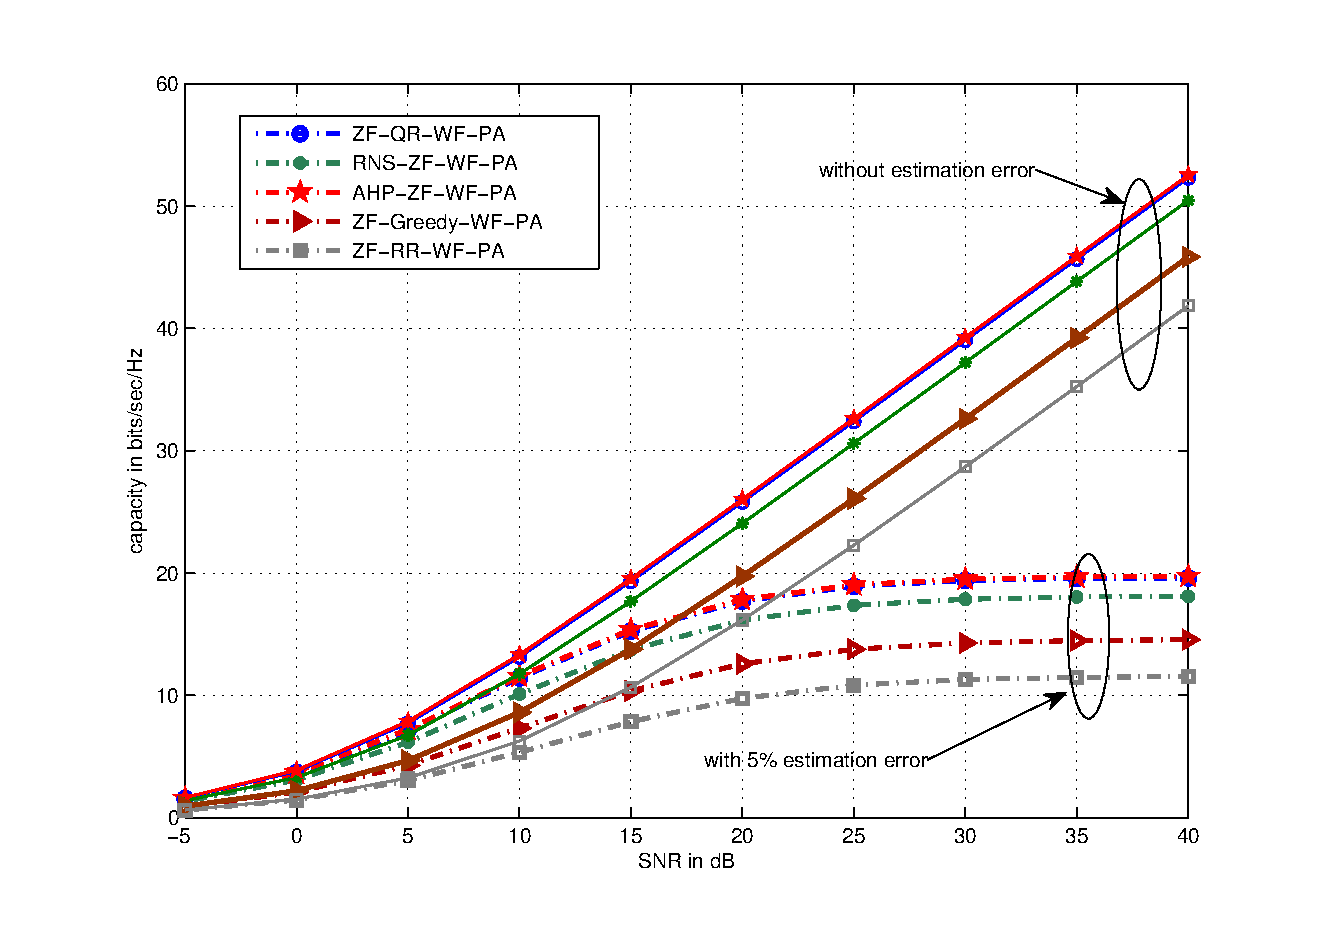
\includegraphics[width=0.8\textwidth]{single-bs-1}
\caption[short]{Sum capacity for \me{\card{\mc{U}} = 20, \, N_\mrm{T} = 4, \, N_\mrm{R} = 1}}
\label{single-bs-f1}
\end{figure}

Fig. \ref{single-bs-f1} compares the performance of capacity achieving user selection schemes discussed in section \ref{mtbus} to the QR based user selection scheme discussed in \cite{antti_user_selection,jin2010novel}. The AHP based user selection provides marginal but still noticeable performance improvement over the existing QR based algorithm. The gain is mainly attributed to the selection mechanism which takes pair-wise channel correlation metric in to account. This additional information is not of great value as it can be seen but the complexity involved in this is significantly large.
\begin{figure}
\centering
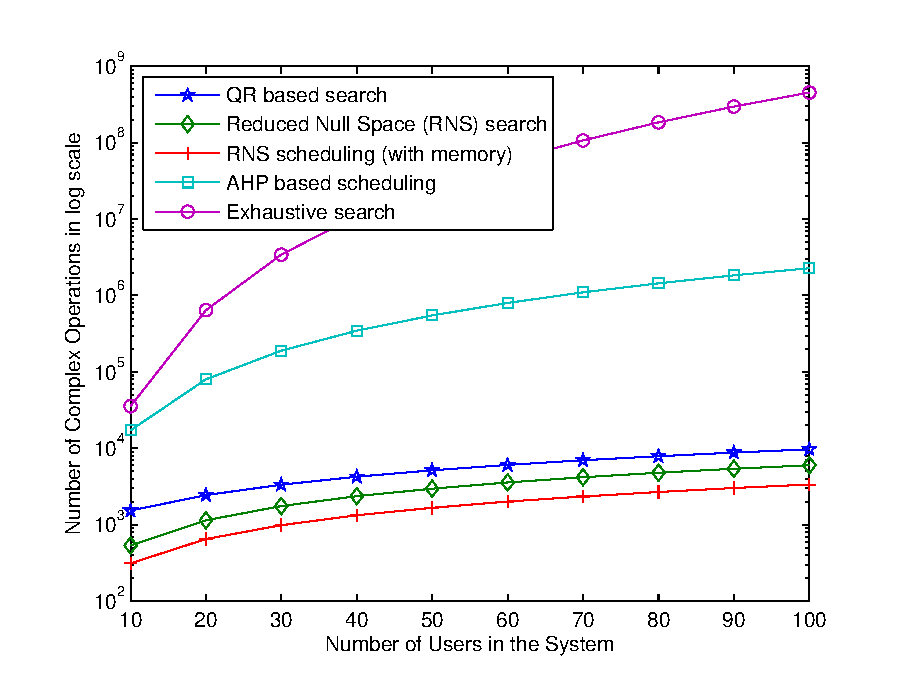
\includegraphics[width=0.8\textwidth]{single-bs-2}
\caption[short]{Scaling of complexity over users for \me{N_\mrm{T} = 4, \, N_\mrm{R} = 1} system}
\label{single-bs-f2}
\end{figure}

Fig. \ref{single-bs-f1} also shows the performance of reduced null space (RNS) scheme which performs closer to the existing QR algorithm but with huge reduction in the complexity involved in the metric calculation. Since QR based schemes requires matrix inverse computation for null space, RNS scheme provides a sub-optimal alternative to achieve the same. Fig. \ref{single-bs-f2} compares the complexity involved in performing various schemes discussed so far. The complexity involved in RNS user selection scheme is the least among the scheduling schemes based on channel correlation discussed here. The complexity can further be reduced by saving the earlier results in the memory (with some increase in the storage memory) to avoid redundant calculations over each iterations.

Fig. \ref{single-bs-f1} depicts the performance degradation of above mentioned schemes with \me{5\%} estimation error modeled using Gaussian error. The estimation error degrades the performance by altering the precoders from being the perfect channel inverse there by creating interference among the transmitted streams. This effect is more pronounced at higher SNR as the capacity is starts saturating since the noise component is dominated by the interference in comparison with the AWGN.
